\chapter{Software}

    \section{Projektstruktur}
    Die Projektstruktur orientiert sich an PlatformIO:
    
    \vspace{0.5cm}
    \begin{minipage}{0.48\linewidth}
            \centering
            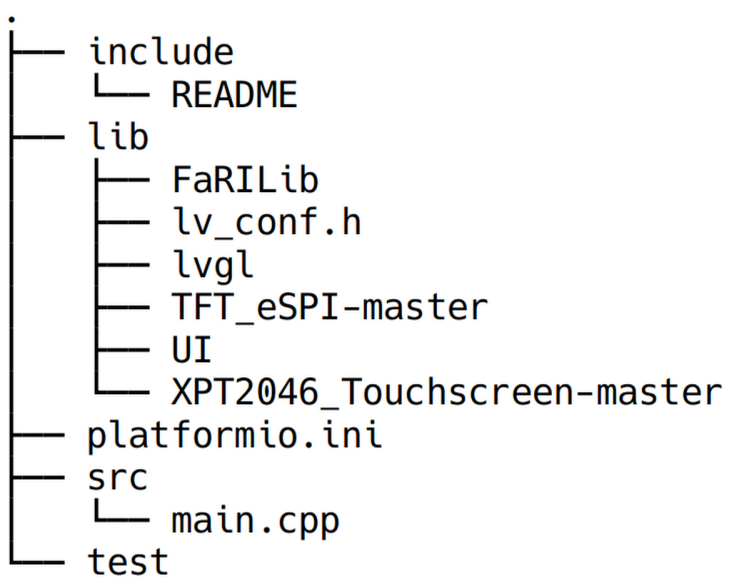
\includegraphics[width=8cm]{projDir}
            \label{fig:projDir}
    \end{minipage}
    \hfill
    \begin{minipage}{0.48\linewidth}
        \raggedright
        \begin{itemize}
            \item custom Libraries werden im \lstinline{lib/} 
            Verzeichnis abgelegt
            \item Libery-unabhängige Header-Dateien 
            werden im \lstinline{include/} Verzeichnis abgelegt
            \item Libery-unabhängige Source-Dateien 
            werden im \lstinline{src/} Verzeichnis abgelegt
        \end{itemize}
    \end{minipage}
    \vspace{0.5cm}

    Während Libraries, die speziell für das Projekt entwickelt oder abgeändert wurden,
    im \lstinline{lib/} Verzeichnis abgelegt werden, werden Libraries,
    die von PlatformIO bereitgestellt werden, automatisch heruntergeladen
    und im verstecktem \lstinline{.pio/} Verzeichnis abgelegt. Diese sind im
    \lstinline{platformio.ini} File spezifiziert.

    \section{FaRiLib}
    Die Libary soll als Grundgerüst für die Implementierung aller Smarthome-Geräte
    dienen. Daher ist der größte Teil der geschriebenen Funktionen Teil der 
    \textit{FaRiLib} Library. Diese Funktionen werden nach Kategorien in verschiedene
    Dateien aufgeteilt (Zum Beispiel: \lstinline{FaRiLib/src/Display.cpp} und 
    \lstinline{FaRiLib/src/ESP-NOW.cpp}). Die selbe Gliederung gilt für die 
    dazugehörigen Header-Dateien (Zum Beispiel: \\ \lstinline{FaRiLib/include/Display.h} und 
    \lstinline{FaRiLib/include/ESP-NOW.h}).

    \section{ESP32-S3 Konfiguration}
    Die Eigenschaften des ESP32-S3 werden in dem \lstinline{platformio.ini}
    File konfiguriert. Als Basis der Konfiguration dient
    das \lstinline{esp32-s3-devkitc-1.json} File, welches die
    Basiskonfiguration für ein ESP32-S3 Devkit bereitstellt
    und standardmäßig von PlatformIO verfügbar ist. \par
    
    Nun müssen folgende Flags im \textit{platformio.ini} File
    überschrieben werden:

    \begin{lstlisting}
    board_upload.flash_size = 16MB
    board_build.partitions = default_16MB.csv
    \end{lstlisting}

    Nun sollte der Upload eines Programms auf den 
    ESP-Chip möglich sein.

    \section{User Interface}
        \subsection{SquarelineStudio}
        SquarelineStudio ist eine Software, die es ermöglicht, ein 
        User Interface mithilfe eines Drag-and-Drop-Editors zu erstellen und
        in C-Code zu exportieren. Dieser Code kann dann dann zusammen mit den 
        beiden Libraries \textit{TFT\_eSPI} und \textit{lvgl} in PlatformIO
        integriert werden.

            \subsubsection{TFT\_eSPI}
            TFT\_eSPI ist eine Library für Grafik und Fonts auf einem TFT-Display.
            Sie ist mit vielen verschiedenen Controllern kompatibel und bietet
            viele Funktionen, um verschiedene TFT-Display anzusteuern.
            Sie ist eine Hälfte des Grundgerüsts für die Darstellung von Grafiken 
            in SquarelineStudio.

            \subsubsection{lvgl}
            lvgl ist eine Library für die Darstellung von flexiblen Grafiken
            auf vielen Platformen, darunter auch dem Arduino Framework.
            Zusammen mit TFT\_eSPI bildet sie das Grundgerüst für die Darstellung
            von Grafiken in SquarelineStudio.
        \subsection{Touch Control}
        Die \textit{TFT\_eSPI} Library bietet auch die Möglichkeit, Touch-Events
        zu registrieren und für das \textit{SquarelineStudio} User Interface zu
        verarbeiten. Diese Funktion ist allerdings nur für über SPI angesteuerte
        Displays verfügbar.
            \subsubsection{XPT2046\_Touchscreen Library}
            Um den Touch seriell einzulesen, wird die \textit{XPT2046\_Touchscreen}
            Library verwendet. 

            \begin{lstlisting}
    #define CS_PIN  10

    XPT2046_Touchscreen ts(CS_PIN);
    TS_Point p;
            \end{lstlisting}

            \subsubsection{Touch mit tft\_eSPI kuppeln} \label{touch_to_tft}
            Um die Touch-Events an tft\_eSPI weiterzuleiten, muss die library grundliegend \\ 
            umgeschrieben werden.
            zunächst muss das User\_Setup.h folgender Maßen bearbeitet werden:

            \begin{lstlisting}
    //Einkommentieren
    #define TOUCH_CS 10 
            \end{lstlisting}

            
            \begin{minipage}{\linewidth}
            Ebenso muss im "tft\_eSPI.h" folgendes editiert werden:
            \begin{lstlisting}   
    #ifdef TOUCH_CS
    //CHANGE THIS LINE
    #if 0
        #if !defined(DISABLE_ALL_LIBRARY_WARNINGS)
        #error >>>>------>> ...
        #endif
    #else
        #include "Extensions/Touch.h"
    #endif
    #else
        #if !defined(DISABLE_ALL_LIBRARY_WARNINGS)
        #warning >>>>------>> ...
        #endif
    #endif
            \end{lstlisting}\end{minipage}
            
            

            \begin{minipage}{\linewidth}
            Nun kann der Touch in der my\_touchpad\_read() Funktion der tft\_eSPI Library
            übergeben werden.
            \begin{lstlisting}
    void my_touchpad_read
    (lv_indev_drv_t*indev_driver, lv_indev_data_t*data)
    {
        uint16_t touchX = 0, touchY = 0;
    
        if( !ts.touched() || p.z < 1950 )
        {
            data->state = LV_INDEV_STATE_REL;
        }
        else
        {
            data->state = LV_INDEV_STATE_PR;
    
            p = ts.getPoint();

            /*Set the coordinates*/
            data->point.x = p.x;
            data->point.y = p.y;
    
            Serial.print( "Data x " );
            Serial.println(data->point.x-700);
    
            Serial.print( "Data y " );
            Serial.println(data->point.y);
        }
    }
            \end{lstlisting}\end{minipage}

            \subsubsection{Touch wurde nicht implementiert}
            Die tft\_eSPI Library verhindert duch die in section \ref{touch_to_tft} 
            beschriebenen \lstinline{#if} Makros, die Implementierung des Touches.
            Trotz mehrerer Versuche, die Library zu modifizieren, wirf die library
            immer wieder \lstinline{include-Fehler} in dem dann inkludierem Touch.h file. \\~\\
            

            


    \section{Kommunikation}
    \subsection{MQTT}
        Um eine Kommunikation zu ermöglichen, ist eine 
        MQTT-Library notwendig. Hierfür wurde "PubSubClient" von 
        "knolleary" verwendet. Hierbei handelt es sich um eine 
        simple Library, die nur das Nötigste implementiert, um
        einen überschaubaren Overhead zu gewährleisten.
    \subsection{ESP-NOW}




